% rotate-copy.tex

\documentclass[tikz]{standalone}
\usetikzlibrary{shapes.multipart, positioning}

\begin{document}
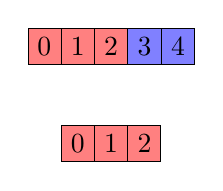
\begin{tikzpicture}[array/.style = {
    rectangle split, rectangle split parts = #1, 
    rectangle split horizontal, 
    rectangle split part fill = {red!50, red!50, red!50, blue!50, blue!50},
    draw, anchor = center, minimum width = 0.60cm}]
  \node (a) [array = 5] {0\nodepart{two}1\nodepart{three}2\nodepart{four}3\nodepart{five}4};

  \node (tmp) [array = 3, below = of a.center] 
    {0\nodepart{two}1\nodepart{three}2};
\end{tikzpicture}
\end{document}